%% 
%% Copyright 2019-2024 Elsevier Ltd
%% 
%% Version 2.4
%% 
%% This file is part of the 'CAS Bundle'.
%% --------------------------------------
%% 
%% It may be distributed under the conditions of the LaTeX Project Public
%% License, either version 1.2 of this license or (at your option) any
%% later version.  The latest version of this license is in
%%    http://www.latex-project.org/lppl.txt
%% and version 1.2 or later is part of all distributions of LaTeX
%% version 1999/12/01 or later.
%% 
%% The list of all files belonging to the 'CAS Bundle' is
%% given in the file `manifest.txt'.
%% 
%% Template article for cas-dc documentclass for 
%% double column output.

%\documentclass[a4paper,fleqn,longmktitle]{cas-dc}
\documentclass[a4paper,fleqn]{cas-sc}

%\usepackage[authoryear,longnamesfirst]{natbib}
%\usepackage[authoryear]{natbib}
\usepackage[numbers]{natbib}

%%%%%%%%%%%%%%%%%%%%
\usepackage{bm}
\usepackage[T1]{fontenc}
% \usepackage{cite}
\usepackage{graphicx}
\usepackage{amsmath}
\usepackage{amsfonts}
\usepackage{amssymb}
\usepackage{tikz}          % to draw vector graphics (figures)
\usetikzlibrary{arrows, shapes, positioning, calc, angles, quotes, arrows.meta} % TikZ libraries for enhanced drawing features
\usepackage{ifthen}
\usepackage{tabularx}
% \usepackage{siunitx} % For number formatting with commas
\usepackage{caption}
\usepackage{pgfplots}
\usepackage{subcaption}
% \usepackage{natbib}
\usepackage[table]{xcolor}
\usepackage{url}
\usepackage{import}
%%%%%%%%%%%%%%%%%%%%

%%%Author definitions
\def\tsc#1{\csdef{#1}{\textsc{\lowercase{#1}}\xspace}}
\tsc{WGM}
\tsc{QE}
\tsc{EP}
\tsc{PMS}
\tsc{BEC}
\tsc{DE}
%%%

\begin{document}
\let\WriteBookmarks\relax
\def\floatpagepagefraction{1}
\def\textpagefraction{.001}
\shorttitle{GPU-accelerated Plane Graph Region Extraction Algorithms}
\shortauthors{Hatem Mira et~al.}

\title [mode = title]{GPU-accelerated Plane Graph Region Extraction Algorithms}


\author[1]{Hatem Mira}
[orcid=0009-0004-0238-4922]
% \fnmark[1]
\cormark[1]
\ead{hmira@aucegypt.edu}

%\address[1]{, Street 129, 1043 NX Amsterdam, The Netherlands}
\affiliation[1]{organization={Department of Computer Science and Engineering, The American University in Cairo},
                city={Cairo},
                country={Egypt}}

\author[1]{Cherif Salama}
[orcid=0000-0002-6986-4697]
\cormark[2]
\ead{cherif.salama@aucegypt.edu}


\cortext[cor1]{Corresponding author}
\cortext[cor2]{Principal corresponding author}
% \fntext[fn1]{This is the first author footnote, but is common to third
%   author as well.}
% \fntext[fn2]{Another author footnote, this is a very long footnote and
%   it should be a really long footnote. But this footnote is not yet
%   sufficiently long enough to make two lines of footnote text.}

% \nonumnote{This note has no numbers. In this work we demonstrate $a_b$
%   the formation Y\_1 of a new type of polariton on the interface
%   between a cuprous oxide slab and a polystyrene micro-sphere placed
%   on the slab.
%   }

\begin{abstract}
This paper presents two high-performance GPU-accelerated algorithms for the extraction of connected regions in plane graphs implemented using the CUDA programming model. While sequential algorithms for extracting all regions of a plane graph $G(V, E)$, with $m$ edges, achieve an optimal time complexity of $O(m \log m)$, they remain constrained by CPU throughput when processing large-scale datasets, and although established libraries such as the Boost Graph Library and the Computational Geometry Algorithms Library provide robust CPU-based solutions, a dedicated GPU implementation currently does not exist in the literature. We introduce a parallel framework that leverages GPUs to exploit the massive parallelism inherent in edge sorting and face traversal.  Experimental results demonstrate that our fastest CUDA-based approach significantly outperforms state-of-the-art CPU implementations, achieving a speedup of up to $33\times$ in total computation time.
\end{abstract}


\begin{keywords}
Plane Graph \sep Region Extraction \sep  Computational Geometry \sep Meshing \sep GPU \sep CUDA \sep CAD
\end{keywords}


\maketitle

\section{Introduction}

A plane graph is a specific topological embedding of a planar graph in a two-dimensional Euclidean space, where vertices are mapped to distinct coordinates and edges are mapped to continuous arcs that intersect exclusively at their common endpoints. Identifying and extracting the discrete regions (or faces) bounded by these edges is a fundamental operation across an extensive array of domains, including geographic information systems (GIS), computer graphics, VLSI layout verification, mesh generation, and automated robotics navigation~\cite{ANTOLIN2023103448,DEMAGALHAES2020102801,10.1145/3139958.3140001}. In modern computational engineering, simulations involving finite element analysis or fluid dynamics frequently manipulate structural meshes containing tens of millions of distinct elements~\cite{Lintermann2021,LINTERMANN2014131,electronics14153151}. At this scale, serial or poorly parallelized geometric extraction routines quickly become severe computational bottlenecks.

% The first optimal sequential algorithm for region extraction that will bed discussed in the paper was proposed Mark de Berg et al~\cite{deberg2008computational} and it is based on Doubly Connected Edge List (DCEL) data structure and the second was proposed by Jiang and Bunke~\cite{JIANG1993553} and is based in Wedges data structure. To differentiate between them the algorithm will be called DCEL-based and Wedge-based algorithms, respectively. Both of them are achieving a time complexity of \(O(m \log m)\) and space complexity of \(O(m)\), where \(m\) is the number of edges in the graph \(G(V, E)\). As shown by Euler's formula for planar graphs, a simple plane graph with \(n \geq 3\) vertices has at most \(m \leq 3n - 6\) edges~\cite{Diestel2025}.

Two primary optimal sequential algorithms for region extraction are discussed in this paper. The first one~\cite{JIANG1993553} is based on wedges, while the second one~\cite{deberg2008computational} is based on half-edges (HEs) and is implemented in many computational geometry libraries, such as the Computational Geometry Algorithms Library (CGAL)~\cite{10.1145/1653771.1653865} and the Boost Graph Library (BGL)~\cite{10.5555/504206}. In this paper, these approaches are referred to as the Wedge-based and HE-based algorithms, respectively. Both methods achieve a time complexity of $O(m \log m)$ and a space complexity of $O(m)$, where $m$ denotes the number of edges in the graph $G(V, E)$. As shown by Euler's formula for planar graphs, a simple plane graph with $n \geq 3$ vertices has at most $m \leq 3n - 6$ edges \cite{Diestel2025}, confirming that such graphs are inherently sparse.

Although theoretically optimal, the original sequential algorithms can be computationally impractical when applied to large-scale graphs commonly encountered in modern scientific and engineering applications, and the emergence of massively parallel platforms, such as GPUs with NVIDIA's CUDA~\cite{10.1145/1401132.1401152} framework, creates new opportunities for accelerating algorithmic graph operations.

% In this paper, we propose a CUDA-based GPU implementation of the optimal region extraction algorithm for plane graphs, emphasizing the design of data structures and execution strategies optimized for GPU architectures. The GPU implementation is evaluated against different reference CPU versions based on the Computational Geometry Algorithms Library (CGAL)~\cite{10.1145/1653771.1653865}, the Boost Graph Library (BGL)~\cite{10.5555/504206}, and our own implementation of the algorithms, using a suite of synthetic 2D mesh datasets that simulate various planar graph structures. Experimental results confirm that the GPU implementation maintains correctness while achieving a substantial speedup compared to the CPU baseline. These findings highlight the effectiveness of parallelization for graph-based geometric processing tasks and demonstrate the practicality of the approach for large-scale applications.

This paper introduces comprehensive GPU-accelerated parallel adaptations of both the Wedge-based and the Half-Edge-based region extraction algorithms. We evaluate our parallel CUDA C++ implementations against established CPU geometric frameworks, including CGAL and BGL, as well as heavily optimized sequential baselines. Our parallel designs adapt a parallel pointer-jumping (path doubling)~\cite{jaja1992} technique and leverage the parallel primitives of the Thrust library~\cite{BELL2012359}. We utilize a suite of synthetic 2D mesh datasets to simulate the large-scale planar graph structures encountered in modern engineering. Experimental results demonstrate that our GPU implementations maintain absolute correctness while achieving substantial speedups—up to 33$\times$ in our tests—compared to CPU baselines. These findings highlight the effectiveness of parallelization for geometric graph processing and demonstrate the practicality of our approach for large-scale applications.

The remainder of this work is structured as follows. Section~\textsc{ii} formalizes the necessary mathematical definitions and structural notations. Section~\textsc{iii} outlines the operational logic of the baseline sequential algorithms. Section~\textsc{iv} provides a deep overview of our proposed parallelization methodologies and CUDA implementation strategies. Section~\textsc{v} presents the experimental results, performance characteristics, and workload profiling, and Section~\textsc{vi} concludes the paper.

\section{Definitions and Notations}


\textbf{Planar Graph:} A graph $G = (V, E)$ is defined as \textit{planar} if it can be drawn on the Euclidean plane $\mathbb{R}^2$ without any edges crossing except at their endpoints (vertices). The term describes a topological property of the graph itself rather than a particular drawing of it. In other words, a graph is called planar if there exists at least one way to represent it in the plane so that no two edges intersect improperly.

It is crucial to distinguish the graph's inherent planarity from its visual representation; a planar graph may be rendered with edge crossings in a given drawing, yet it remains planar as long as at least one crossing-free configuration exists. Conversely, \textit{non-planar graphs} cannot be drawn without at least one intersection, regardless of the arrangement. The most fundamental examples of non-planar graphs are the complete graph $K_5$ and the complete bipartite graph $K_{3,3}$ shown in Figure~\ref{fig:nonplanar}.

\begin{figure}
\centering
% ----------- K5 -----------
\begin{subfigure}[t]{0.45\linewidth}
\centering
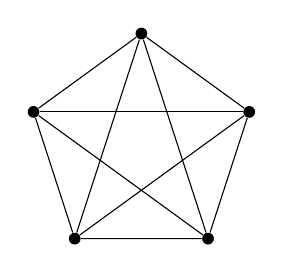
\begin{tikzpicture}[scale=1.2, every node/.style={circle, fill=black, inner sep=1.5pt}]
    \foreach \i in {1,...,5}
        \node (v\i) at ({90-(\i-1)*72}:1.2) {};
    
    \draw (v1)--(v2)--(v3)--(v4)--(v5)--(v1);
    \draw (v1)--(v3);
    \draw (v1)--(v4);
    \draw (v2)--(v4);
    \draw (v2)--(v5);
    \draw (v3)--(v5);
\end{tikzpicture}
\caption{The complete graph $K_5$}
\end{subfigure}
\hfill
% ----------- K3,3 -----------
\begin{subfigure}[t]{0.45\linewidth}
\centering
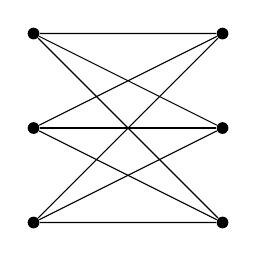
\begin{tikzpicture}[scale=1.2, every node/.style={circle, fill=black, inner sep=1.5pt}]
    \foreach \i in {1,2,3} {
        \node (a\i) at (0, \i-2) {};
        \node (b\i) at (2, \i-2) {};
    }
    \foreach \i in {1,2,3}
        \foreach \j in {1,2,3}
            \draw (a\i)--(b\j);
\end{tikzpicture}
\caption{The bipartite graph $K_{3,3}$}
\end{subfigure}
\caption{The two minimal non-planar graphs shown with unavoidable edge crossings.}
\label{fig:nonplanar}
\end{figure}

\textbf{Plane Graph:} While "planar" refers to the capacity of the graph to be drawn without crossings, a \textit{plane graph} refers to a specific \textit{planar embedding} (or drawing) of that graph in which no two edges intersect except at their endpoints. 

As illustrated by the complete graph $K_4$ in Figure~\ref{fig:k4_example}, a single planar graph can yield multiple representations. A drawing of $K_4$ in a standard rectilinear format typically results in an edge crossing; however, by relocating a single vertex or routing an edge externally, a crossing-free "plane" representation is achieved. This demonstrates that while $K_4$ is fundamentally a planar graph, only specific drawings of it constitute plane graphs.

\begin{figure}
\centering
% ----------- Planar embedding of K4 -----------
\begin{subfigure}[t]{0.45\linewidth}
\centering
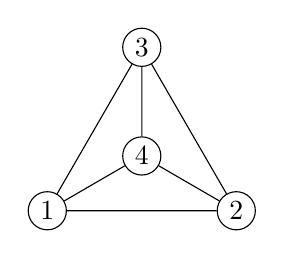
\begin{tikzpicture}[scale=1.2, every node/.style={circle, draw, fill=white, inner sep=2pt}]
    \node (v1) at (0,0) {1};
    \node (v2) at (2,0) {2};
    \node (v3) at (1,1.73) {3};
    \node (v4) at (1,0.58) {4};
    
    \draw (v1)--(v2)--(v3)--(v1);
    \draw (v1)--(v4);
    \draw (v2)--(v4);
    \draw (v3)--(v4);
\end{tikzpicture}
\caption{A plane embedding of $K_4$}
\label{fig:k4_planar}
\end{subfigure}
\hfill
% ----------- Non-planar drawing of K4 -----------
\begin{subfigure}[t]{0.45\linewidth}
\centering
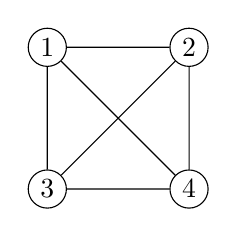
\begin{tikzpicture}[scale=1.2, every node/.style={circle, draw, fill=white, inner sep=2pt}]
    \node (v1) at (0,1.5) {1};
    \node (v2) at (1.5,1.5) {2};
    \node (v3) at (0,0) {3};
    \node (v4) at (1.5,0) {4};
    
    \draw (v1)--(v2)--(v4)--(v3)--(v1);
    \draw (v1)--(v4);
    \draw (v2)--(v3);
\end{tikzpicture}
\caption{A non-plane drawing of $K_4$}
\label{fig:k4_nonplanar}
\end{subfigure}
\caption{Verification of the planarity of $K_4$: (a) provides a valid plane embedding, while (b) illustrates a drawing with a crossing that does not alter the graph's underlying planarity.}
\label{fig:k4_example}
\end{figure}


A plane graph divides the plane into distinct areas called \emph{regions} (also known as \emph{faces}, \emph{windows}, or \emph{meshes}). Each region is defined by the set of edges forming its boundary. For example, the graph shown in Figure~\ref{fig:plane_graph} contains three such regions:

\begin{align*}
R_1 = (&(v_1, v_2), (v_2, v_4), (v_4, v_5), (v_5, v_6), (v_6, v_1)) \\
R_2 = (&(v_1, v_6), (v_6, v_3), (v_3, v_1)) \\
R_3 = (&(v_1, v_3), (v_3, v_6), (v_6, v_5), (v_5, v_4), (v_4, v_2), \\
&(v_2, v_1))
\end{align*}


\begin{figure}
    \centering
    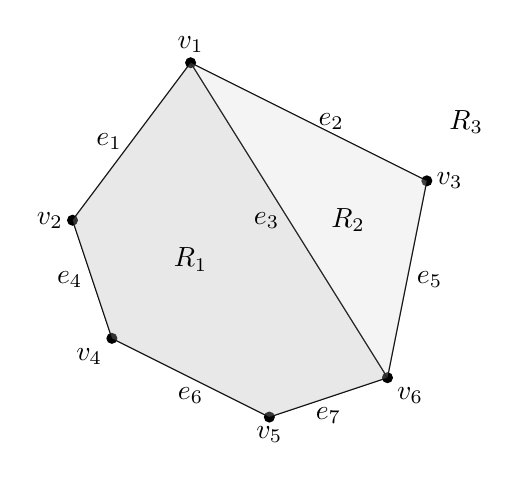
\begin{tikzpicture}
        % vertices
        \coordinate (v1) at (0,4.5);
        \coordinate (v2) at (-1.5,2.5);
        \coordinate (v3) at (3,3);
        \coordinate (v4) at (-1,1);
        \coordinate (v5) at (1,0);
        \coordinate (v6) at (2.5, 0.5);
        
        % edges
        \draw (v1) -- (v2);
        \draw (v1) -- (v6);
        \draw (v3) -- (v1);
        \draw (v2) -- (v4);
        \draw (v4) -- (v5);
        \draw (v5) -- (v6);
        \draw (v6) -- (v3);
        
        % labels with math mode
        \foreach \v/\pos/\labeltext in {v1/above/$v_1$, v2/left/$v_2$, v3/right/$v_3$, v4/below left/$v_4$, v5/below/$v_5$, v6/below right/$v_6$}
        {    
            \node[\pos] at (\v) {\labeltext};
            \fill (\v) circle[radius=2pt];  % black filled circle
        }
        
        % regions - lightly shaded for clarity
        \begin{scope}
            \filldraw[fill=gray!60,opacity=0.3] (v1) -- (v2) -- (v4) -- (v5) -- (v6) -- cycle;
            \filldraw[fill=gray!30,opacity=0.3] (v1) -- (v6) -- (v3) -- cycle;
            % The exterior region outside edges can be left unshaded
        \end{scope}
            
        % edge labels (midpoints)
        \node[left] at ($(v1)!0.5!(v2)$) {$e_1$};
        \node[right] at ($(v1)!0.5!(v3)$) {$e_2$};
        \node[left] at ($(v1)!0.5!(v6)$) {$e_3$};
        \node[left] at ($(v2)!0.5!(v4)$) {$e_4$};
        \node[right] at ($(v3)!0.5!(v6)$) {$e_5$};
        \node[below] at ($(v5)!0.5!(v4)$) {$e_6$};
        \node[below] at ($(v5)!0.5!(v6)$) {$e_7$};
        
        % region labels (inside faces)
        \node at (0,2) {$R_1$}; % triangle top region
        \node at (2,2.5) {$R_2$};   % quadrilateral below
        \node at (3.5,3.75) {$R_3$}; % exterior region (optional)
        
    \end{tikzpicture}
    \caption{Plane graph with seven edges forming three regions.}
    \label{fig:plane_graph}
\end{figure}

Among them, \( R_3 \) is called the \emph{exterior region}, which lies outside the boundary of the graph.
Given two edges \( e_1 = (v_i, v_j) \) and \( e_2 = (v_j, v_k) \); if rotating \( e_1 \) in a clockwise direction around the shared vertex \( v_j \) toward \( e_2 \) does not encounter any other edge incident on \( v_j \), then the area enclosed between \( e_1 \) and \( e_2 \) defines a \emph{wedge}, denoted \( (v_i, v_j, v_k) \). Two wedges such as \( (v_i, v_j, v_k) \) and \( (v_j, v_k, v_l) \) are called contiguous.
In any plane graph with \( m \) edges, there are exactly \( 2m \) wedges. Returning to the graph in Figure~\ref{fig:plane_graph}, which has 7 edges, we find 14 wedges:
\begin{align*}
& (v_2, v_1, v_3),\ (v_3, v_1, v_6),\ (v_6, v_1, v_2),\ (v_4, v_2, v_1), \\
&  (v_1, v_2, v_4),\ (v_1, v_3, v_6),\ (v_6, v_3, v_1),\ (v_2, v_4, v_5), \\
& (v_5, v_4, v_2),\ (v_4, v_5, v_6),\ (v_6, v_5, v_4),\ (v_1, v_6, v_3), \\
& (v_3, v_6, v_5),\ (v_5, v_6, v_1)
\end{align*}
Each region in a plane graph can be represented in any one of the three equivalent ways:
\begin{itemize}
    \item As a sequence of \emph{vertices}
    \item As a sequence of \emph{edges}
    \item Or as a sequence of \emph{wedges}.
\end{itemize}
For example, region \( R_1 \) from Figure~\ref{fig:plane_graph} can be expressed as:
\begin{align*}
(&v_1, v_2, v_4, v_5, v_6), \\
(&(v_1, v_2), (v_2, v_4), (v_4, v_5), (v_5, v_6), (v_6, v_1)), \text{ or } \\
(&(v_1, v_2, v_4), (v_2, v_4, v_5), (v_4, v_5, v_6), (v_5, v_6, v_1),\\
&(v_6, v_1, v_2))
\end{align*}
The three representations are equivalent and can be easily transformed into each other. Thus, either of them can be chosen for convenience.

\textbf{Half-Edge:} In the context of computational geometry, a half-edge is a directed representation of an edge. It is like a general directed edge, but additionally, it points to the next half-edge, which allows a "walk" around any polygon.

\textbf{Twin Edge:} Every half-edge $e = \langle u, v \rangle$ that originates at the vertex $u$ and ends at the vertex $v$ is associated with a unique \textit{twin edge} $\bar{e} = \langle v, u \rangle$. The twin edge originates at $v$ and ends at $u$, representing the same geometric span but oriented in the opposite direction. Figure~\ref{fig:half_edges} illustrates half-edges and their twin edges of a triangle.

\begin{figure}
    \centering
    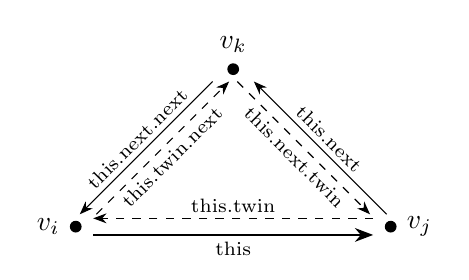
\begin{tikzpicture}[
        vertex/.style={circle, fill=black, inner sep=1.5pt},
        thisedge/.style={->, >=Stealth, shorten >=4pt, thick, shorten <=4pt},
        halfedge/.style={->, >=Stealth, shorten >=4pt, shorten <=4pt},
        twinedge/.style={->, >=Stealth, shorten >=4pt, dashed, shorten <=4pt},
        % nextarrow/.style={->, >=latex, dashed, orange}
        nextarrow/.style={->, orange},
        edgeLabel/.style={midway, sloped, font=\scriptsize, inner sep=2pt}
    ]
        % Vertices
        \node[vertex, label=left:$v_i$] (vi) at (0,0) {};
        \node[vertex, label=right:$v_j$] (vj) at (4,0) {};
        \node[vertex, label=above:$v_k$] (vk) at (2, 2) {};

        % Half-edges (twins)
        \draw[thisedge, transform canvas={yshift=-3pt}] (vi) -- (vj) node[edgeLabel, below] {this};
        \draw[twinedge, transform canvas={yshift=3pt}] (vj) -- (vi) node[edgeLabel, above] {this.twin};

        \draw[halfedge, transform canvas={xshift=3pt}] (vj) -- (vk) node[edgeLabel, above] {this.next};
        \draw[twinedge, transform canvas={xshift=-3pt}] (vk) -- (vj) node[edgeLabel, below] {this.next.twin};

        \draw[halfedge, transform canvas={xshift=-3pt}] (vk) -- (vi) node[edgeLabel, above] {this.next.next};
        \draw[twinedge, transform canvas={xshift=3pt}] (vi) -- (vk) node[edgeLabel, below] {this.twin.next};        
    \end{tikzpicture}
    \caption{An illustration of half-edges and their twin edges of a triangle}
    \label{fig:half_edges}
\end{figure}

\section{Optimal Sequential Algorithms}
In this section, we illustrate the steps of the optimal sequential algorithms for region extraction (the Wedge-based and the HE-based), which have run-time complexity \( O (m \log m) \) and space complexity \( O (m) \). We will also shed light on the time complexity of each step because it will be the guide to the design of the GPU-accelerated algorithms proposed in the methodology. Both algorithms take as input an undirected connected graph \(G(V, E)\) with a list of vertices \(V\), each vertex \(v_i\) with coordinates \((x_i, y_i)\), and a list of undirected edges \(E\). 


\subsection{The Wedge-based Algorithm}
The algorithm proceeds in two main phases: first, it identifies all possible wedges; next, it groups these wedges to form the regions.
\subsubsection{Phase 1: Wedge Construction}
The first phase identifies all wedges in the input plane graph, which are angular regions formed around each vertex by consecutive incident edges. The steps of this phase are as follows:

\begin{enumerate}
    \item \textbf{Edge Duplication:} Each undirected edge \( (v_i, v_j) \) is duplicated to form two directed edges \( \langle v_i, v_j\rangle \) and \( \langle v_j, v_i\rangle \) representing both directions. This prepares the graph for directional angular computations. Time complexity to duplicate all edges is \( O(m) \).
    \item \textbf{Angle Calculation:} For each directed edge \( \langle v_i, v_j\rangle \), the angle \( \theta\) relative to the positive side of the horizontal axis passing through its source vertex is computed, enabling sorting of edges by their spatial orientation around each vertex. The time complexity of calculating angles for all edges is \( O(m) \).
    \item \textbf{Sorting:} Directed edges \( \langle v_i, v_j\rangle \) are first sorted by their source vertex \( v_i\) and then by their angles \( \theta \). This ensures that edges incident to each vertex are arranged in a counter-clockwise order to allow wedge formation. The time complexity of sorting edges is \( O(m \log m) \). An example of sorting edges by their angles is shown in Figure~\ref{fig:edge_angle_sorting}, where the sorted edges are \(e_i, e_j, e_k\).
    \item \textbf{Wedge Generation:} For each vertex group which has the same source vertex \( v_i \), wedges are constructed by pairing each edge \((\langle v_i, v_j \rangle, \theta_1)\) with its successive neighbor in the group \((\langle v_i, v_k \rangle, \theta_2)\) to build the wedge \( (v_k, v_i, v_j) \), with the last edge paired with the first to complete the cycle. The time complexity of building wedges from the edges is \( O(m) \). In Figure~\ref{fig:edge_angle_sorting} the constructed wedges are \((v_6, v_1, v_2)\, (v_3, v_1, v_6)\, (v_2, v_1, v_3)\).
\end{enumerate}

The time complexity of the first phase is \(O(m \log m)\) because of the sorting step.

\begin{figure}
    \centering
    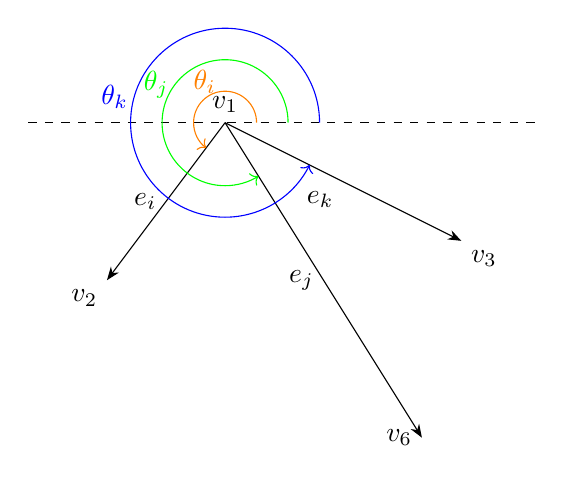
\begin{tikzpicture}
        % vertices
        \coordinate (v1) at (0,4.5);
        \coordinate (v2) at (-1.5,2.5);
        \coordinate (v3) at (3,3);
        \coordinate (v6) at (2.5, 0.5);
        \coordinate (xref) at (1,4.5); % reference point for x-axis direction from v1
        
        % directed edges
        \draw[>=Stealth, ->] (v1) -- (v2);
        \draw[>=Stealth, ->] (v1) -- (v3);
        \draw[>=Stealth, ->] (v1) -- (v6);
        
        \draw[dashed] (-2.5,4.5) -- (4,4.5);
        
        % labels with math mode
        \foreach \v/\pos/\labeltext in {v1/above/$v_1$, v2/below left/$v_2$, v3/below right/$v_3$, v6/left/$v_6$}
            \node[\pos] at (\v) {\labeltext};
        
            
        % edge labels (midpoints)
        \node[left] at ($(v1)!0.5!(v2)$) {$e_i$};
        \node[left] at ($(v1)!0.5!(v6)$) {$e_j$};
        \node[below left] at ($(v1)!0.5!(v3)$) {$e_k$};

         
        % Angles with labels
        \pic [draw=orange, text=orange, ->, "$\theta_i$", angle radius=0.4cm, angle eccentricity=1.45] {angle = xref--v1--v2};
        \pic [draw=green, text=green, ->, "$\theta_j$", angle radius=0.8cm, angle eccentricity=1.25] {angle = xref--v1--v6};
        \pic [draw=blue, text=blue, ->, "$\theta_k$", angle radius=1.2cm, angle eccentricity=1.2] {angle = xref--v1--v3};
        % \pic [draw=green, text=green, ->, "$ \theta_k $, angle radius=0.8cm, angle eccentricity=1.2] {angle = xref--v1--v3};
        % \pic [draw, ->, angle radius=0.6cm, angle eccentricity=1.2, angle label={$ \theta_j $}] {angle = xref--v1--v6};

        
        
    \end{tikzpicture}
    \caption{Sorting Edges according to angle with the horizontal axis. Sorted edges are \( e_i, e_j, e_k\)}
    \label{fig:edge_angle_sorting}
\end{figure}

\subsubsection{Phase 2: Build Regions from Wedges}
The region grouping phase assembles wedges into closed polygonal regions, identifying all face boundaries of the plane graph. It can be easily proven that a region can be defined by a sequence of wedges \( (W_1, W_2, ..., W_k)\) if and only if \( W_i\) and \( W_{i + 1}\) are contiguous for \( i = 1, 2, ..., k - 1\) and also \( W_k\) and \(W_1\) are contiguous. We will depend on that to create the regions according to the following steps:

\begin{enumerate}
    \item \textbf{Sorting Wedges:} Given the list of wedges \( (v_i, v_j, v_k) \) constructed from the first phase, wedges are sorted by \( v_i \) then by \( v_j \). Time complexity is \( O(m \log m) \).
    \item \textbf{Marking Wedges:} Mark all wedges as unvisited wedges. Time Complexity is \( O (m) \).
    \item \label{phase2_start} \textbf{Region Start Wedge:} Each wedge is examined in order. If a wedge has not yet been used to construct a previous region, it is used as the starting wedge \( W_1 \) for constructing a new region, and it is marked as a visited wedge.
    \item \textbf{Contiguous Wedge Search:} In this step, we iterate over the wedges till we define the current region as follows: 
    \begin{enumerate}
        \item \textbf{Binary Search:} Using binary search within the sorted wedge list, the algorithm finds the next contiguous wedge \( W_{i + 1}\) sharing an edge with the current one \( W_i \), extending the region boundary, and the new wedge is marked as a visited wedge. Time complexity of the binary search step is \( O (\log m) \).
        \item \textbf{Closure Detection:} The process continues until the initial wedge is reached again, completing the closed polygonal region.
    \end{enumerate}
    \item \textbf{Completion:} If there is no unvisited wedge, then the phase is completed; otherwise, go back to step~\ref{phase2_start}.
\end{enumerate}
Because every wedge is visited exactly once during the tracing loops, the cumulative cost of the binary searches across all $2m$ wedges is mathematically bounded by $O(m \log m)$. Consequently, when combining the sorting stage with the traversal loop, Phase 2 maintains an overall time complexity of $O(m \log m)$, matching the total asymptotic bounds of the complete extraction algorithm.


\subsection{The HE-based Algorithm}
The algorithm proceeds in two main phases: first, it constructs the half-edges with their next and twin edges from the input graph; next, it traverses the half-edges to extract all regions.

\subsubsection{Phase 1: Half-Edges Construction}
The first phase builds the topological relationships required for the half-edges. The steps are as follows:

\begin{enumerate}
    \item \textbf{Half-Edge Creation:} Each undirected edge $(v_i, v_j)$ is split into two directed \textit{half-edges}, $e_{i,j}$ (originating at $v_i$) and $e_{j,i}$ (originating at $v_j$). Each half-edge is assigned to its twin edge immediately. Time complexity is $O(m)$.
    \item \textbf{Angle Calculation:} For each directed edge \( \langle v_i, v_j\rangle \), the angle \( \theta\) is calculated in a similar way to the step in the Wedge-based algorithm. The time complexity of calculating angles for all edges is \( O(m) \).
    \item \textbf{Angular Sorting:} For every vertex $v$, all half-edges originating at $v$ are sorted by their polar angle ascending. This step is identical to the Wedge-based algorithm, and is required to determine the relative order of edges around a vertex. Time complexity is $O(m \log m)$.
    \item \textbf{Next Edge Linking:} For each half-edge $e_{i,j}$ (which terminates at $v_j$), its next edge must be a half-edge originating at $v_j$. Specifically, the immediate clockwise successor of its twin edge around the vertex $v_j$ (the previous half-edge of its twin edge in the sorted half-edges around $v_j$). This ensures that the traversal follows the boundary of the incident face. The time complexity of linking one edge is $O(1)$ and, hence, for all edges is $O(m)$. A visual example of this step is shown in Figure~\ref{fig:dcel_pointers}, where the next half-edge of $e_{3,1}$ is calculated as $e_{1,6}$ because it is the half-edge that has the largest angle less than its twin edge $e_{1,3}$.
\end{enumerate}

Similar to the Wedge-based approach, the total time complexity of the HE-based algorithm is $O(m \log m)$ due to the sorting requirement.

\begin{figure}
    \centering
    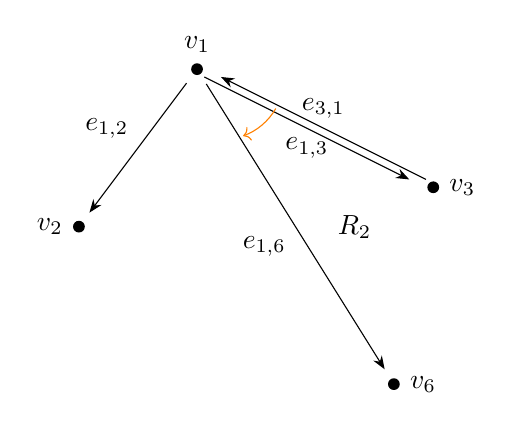
\begin{tikzpicture}[
        vertex/.style={circle, fill=black, inner sep=1.5pt},
        halfedge/.style={->, >=Stealth, shorten >=4pt, shorten <=4pt},
        % nextarrow/.style={->, >=latex, dashed, orange}
        nextarrow/.style={->, orange}
    ]
        % Vertices
        \node[vertex, label=right:$v_3$] (vi) at (3,3) {};
        \node[vertex, label=above:$v_1$] (vj) at (0,4.5) {};
        \node[vertex, label=right:$v_6$] (vk) at (2.5, 0.5) {};
        \node[vertex, label=left:$v_2$] (vl) at (-1.5,2.5) {};

        % Half-edges (twins)
        \draw[halfedge, transform canvas={xshift=3pt}] (vi) -- (vj) node[midway, above] {$e_{3,1}$};
        \draw[halfedge, transform canvas={xshift=-3pt}] (vj) -- (vi) node[midway, below] {$e_{1,3}$};

        % Next pointer visualization
        \draw[halfedge] (vj) -- (vk) node[midway, below left] {$e_{1,6}$};
        \draw[halfedge] (vj) -- (vl) node[midway, above left] {$e_{1,2}$};
        % \draw[->, dashed, bend right, orange] (-1.25, 1.75) to node[right, font=\small] {next} (0, 0.5);
        % \draw[nextarrow] (-1.25, 1.75) to node[above right, font=\small] {next} (0, 0.5);
        % \draw[nextarrow] (0, 0.5) arc (-45 : 135 : 0.4)
        %     node[midway, right, font=\scriptsize, text=orange] {next};
        \draw[nextarrow] (1, 4) arc (330 : 290 : 0.79)
    node[midway, right, font=\small, text=orange]{};

        \node at (2,2.5) {$R_2$};
    \end{tikzpicture}
    \caption{Next Edge Linking. The next edge of $e_{3,1}$ points to the half-edge $e_{1,6}$ based on the angular order around $v_1$.}
    \label{fig:dcel_pointers}
\end{figure}

\subsubsection{Phase 2: Region Traversal}
Once the half-edges with their next and twin edges are calculated, extracting regions becomes a linear-time pointer-following exercise. Unlike the Wedge-based algorithm, no binary search is required in this phase because the topology is explicitly stored.

\begin{enumerate}
    \item \textbf{Initialization:} All half-edges are marked as unvisited. A global list of regions is initialized. Time complexity is $O(m)$.
    \item \textbf{Edge Selection:} The algorithm iterates through the half-edges. If a half-edge $e$ has not been visited, it is selected as the starting edge of a new region.
    \item \textbf{Cycle Traversal:} Starting from $e$, the algorithm follows the next half-edges until the starting half-edge $e$ is reached again. All half-edges encountered in this cycle are marked as visited and added to the current region.
    \item \textbf{Completion:} The process repeats until all half-edges have been visited. 
\end{enumerate}

Since each half-edge is visited exactly once and the time complexity is constant per helf-edge during the traversal, the time complexity of Phase 2 is $O(m)$. Consequently, the overall complexity of the HE-based algorithm is dominated by the sorting in Phase 1, resulting in $O(m \log m)$. Although the HE-based algorithm has the same time complexity as the Wedge-based algorithm, $O(m \log m)$, it does not have the binary search step, and it is expected to have a better run-time performance.

\section{Methodology}
In this section, we will illustrate the GPU-accelerated algorithm for both the wedge-based and the HE-based algorithms.  

\subsection{The Wedge-based Algorithm}
The CUDA-based parallel implementation of the wedge-based algorithm adheres to the two-phase structure originally introduced by Jiang and Bunke~\cite{JIANG1993553}, with necessary adaptations to enable parallel execution. These adaptations include the incorporation of CUDA-specific libraries and the application of parallelization strategies tailored for GPU architectures. The implementation of each phase is detailed as follows:

\subsubsection{Phase 1: Wedge Construction}
The first phase identifies all wedges in the input plane graph. Despite this phase being computationally intensive, it is highly parallelizable and hence well-suited for GPU execution with the use of the Thrust~\cite{BELL2012359} library in CUDA. The Thrust API provides an easy-to-use high-level interface for parallel programming on CUDA-enabled GPUs. It offers a wide range of functionalities such as scan, sort, reductions, and data transformations. 
The computation proceeds as follows:

\begin{itemize}
    \item \textbf{Copy Edges:} Copy the edges data from the CPU to the GPU.
    \item \textbf{Edge Duplication:} Each undirected edge is passed to a thread to get duplicated to form two directed edges representing both directions. This prepares the graph for directional angular computations. This step is fully parallelizable in a direct way by duplicating each edge on a thread.
    \item \textbf{Angle Calculation:} Each directed edge is passed to a thread, then the angle relative to the horizontal axis passing through its source vertex is calculated.  This step is fully parallelizable in a direct way by calculating the angle for each edge on a thread.
    \item \textbf{Sorting:} Directed edges are first sorted by their source vertex and then by their angles. This step is parallelized using the sort function in the Thrust library.
    \item \textbf{Grouping Edges:} The sorted edges are grouped by their source vertices. This step is parallelized using the reduce\_by\_key function in the Thrust library in CUDA, which identifies the groups around each vertex and calculates their sizes.
    \item \textbf{Wedge Generation:} Each vertex group is passed to a thread where wedges are constructed by pairing each edge with its successive neighbor in the group, with the last edge paired with the first to complete the cycle. This step is also parallelizable, with each thread independently processing a group of sorted edges, where the number of iterations per thread corresponds to the number of edges in a group, which is typically much less than \(m\), the total number of edges in the graph.
\end{itemize}

\subsubsection{Phase 2: Build Regions from Wedges}
The region grouping phase assembles wedges into closed polygonal regions, identifying all face boundaries of the plane graph. Unlike the first phase, this phase in the original algorithm requires sequential traversal and dynamic data-dependent operations, which are inherently less amenable to parallelization, but still, this phase is accelerated as illustrated in the following steps of the algorithm.

\begin{enumerate}
    \item \textbf{Wedge Sorting:} The resulting wedges from phase 1 are stored by their vertex pairs for efficient lookup. The sort step is done using the Thrust library in CUDA.
    \item \textbf{Wedge Initialization:} All the wedges are marked as unvisited in preparation for region extraction, each wedge in a thread. This step is fully parallelizable.
    \item \textbf{Search for the contiguous wedges}: In this step, we pass each wedge to a thread and calculate the contiguous wedge for each wedge using binary search, and save this data. As a result, we can, later, find the contiguous wedge for any wedge in constant time. This step is fully parallelizable as each wedge searches for its contiguous wedge in a thread, and the binary search operation has time complexity \(O(\log m)\).
    \item \textbf{Calculate Leaders}: To uniquely identify the regions of the plane graph, we map all wedges belonging to the same region to a single representative identifier. We employ a parallel pointer jumping technique (also known as path doubling) to achieve this convergence efficiently. Let $W$ be the set of $2m$ wedges. Each wedge $w_i \in W$ maintains a successor pointer $S[i]$ and a label $L[i]$. Initially, $S[i]$ is set to the index of the contiguous wedge of $w_i$, and $L[i]$ is initialized to the index $i$. The objective is to reach a steady state where all wedges belonging to the same region $R \subseteq W$ share a uniform label, specifically the minimum index within that region:
    $$\forall i \in R, \quad L[i] = \min_{j \in R} \{j\}$$
    In a sequential environment, identifying the minimum label in a cycle of length $c$ requires $O(c)$ operations. To leverage GPU parallelism, we utilize a geometric progression managed by a host-side loop. In each iteration $k$, a kernel is launched where every wedge is processed by a thread to concurrently update its label and successor by referencing those of its current target:
    $$S_{k+1}[i] = S_k[S_k[i]]$$
    $$L_{k+1}[i] = \min(L_k[i], L_k[S_k[i]])$$
    This doubling effect ensures that by iteration $k$, each wedge has traversed a path of length $2^k$. Consequently, any region of size $c$ is fully traversed in $\lceil \log_2 c \rceil$ iterations. Simultaneously, we perform a reduction-style update on the labels; for each wedge $w_i$, we compare its current label with the label of its successor $S[i]$ and retain the minimum. The loop terminates when no further label updates occur across the wedges. Figure~\ref{fig:pointer_jumping} illustrates the progression of leader values for a region of size 8, with wedge indices ranging from 0 to 7. Initially, each wedge $w_i$ is defined by two properties: $L_0[i] = i$ and $S_0[i] = (i + 1) \pmod{8}$. After iteration 1, $L_1[7]$ is the only updated label, as $w_7$ is the only wedge whose successor has a smaller index. The successors are then updated to $S_1[i] = S_0[S_0[i]] = (i + 2) \pmod{8}$. By iteration 2, both $w_5$ and $w_6$ update their labels, and the successors for all wedges become $S_2[i] = (i + 4) \pmod{8}$. Following the final iteration, all wedges $w_0$ through $w_7$ converge to the label 0.

    % \item \textbf{Construct Regions:} Following convergence, a final kernel is launched to linearize the wedges within each region. In this step, parallelism is exploited at the region level rather than the wedge level; each thread is assigned to a unique region leader and performs a sequential "walk" through the linked wedges. This process begins with the leader and follows the original contiguous pointers until the entire cycle is visited. While this step is sequential within each region, a key advantage of this design is the significant reduction in the required thread count. By scaling the number of threads to the number of regions ($|R|$) rather than the number of wedges ($2m$), the implementation minimizes the overhead associated with thread management and maximizes the availability of hardware resources per active thread. This approach prevents resource over-subscription on the GPU, though it remains sensitive to the distribution of region sizes; the overall execution time is governed by the longest cycle, which becomes the primary computational bottleneck. The pointer jumping technique can also be used here in this step, but in spite of having a logarithmic run time complexity instead of the linear run time complexity of the current implementation, the fact that the pointer jumping needs to run on a $2m$ number of threads simultaneously makes it slower in practice. 

    \item \textbf{Construct Regions:} Following the convergence of region leaders, a kernel is launched to linearize the constituent wedges of each independent region. In this phase, parallelism is exploited at the region level rather than the wedge level; each thread is assigned to a unique region leader and executes a sequential traversal along the original contiguous pointers, starting from the leader, until the boundary cycle is fully reconstituted. 

    While the traversal within each region is sequential, this design minimizes resource utilization by scaling the active thread count to the number of discrete regions ($|R|$) rather than the total number of wedges ($2m$). This reduction in thread density mitigates thread management overhead, prevents GPU resource over-subscription, and maximizes the execution context resources available per active thread.
    
    Although using pointer jumping would yield a logarithmic time complexity of $O(\log c)$ for a cycle of length $c$, it requires maintaining a thread allocation scaled to all $2m$ wedges. Consequently, the linear traversal over $|R|$ threads proves more efficient in practice due to reduced kernel launch overhead, even though its execution time remains bounded by the maximum cycle length, $O(\max c)$.
    
    \item \textbf{Copying Regions:} Copy the regions data back to the CPU.
\end{enumerate}

\begin{figure}
\centering
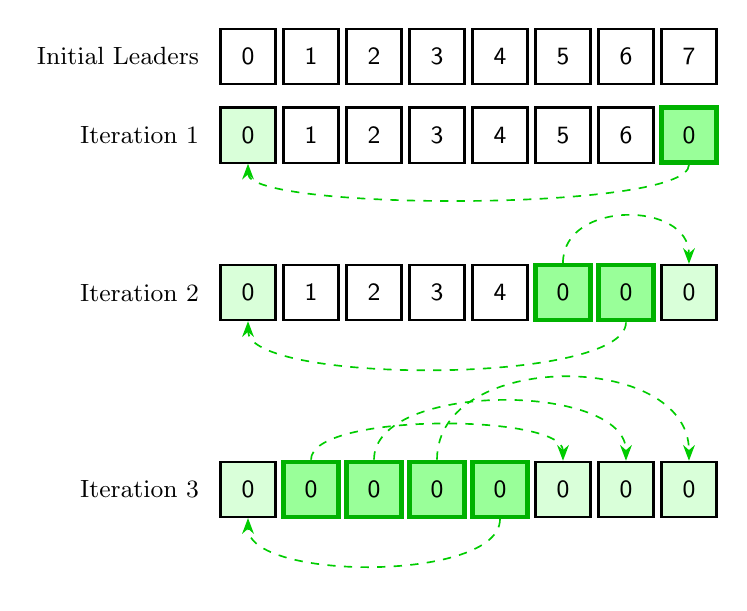
\begin{tikzpicture}[
    every node/.style={font=\small\sffamily},
    box/.style={draw, thick, minimum size=0.7cm, anchor=center},
    new_leader/.style={fill=green!40, draw=green!70!black, ultra thick},
    old_leader/.style={fill=green!15},
    jump/.style={->, >=Stealth, semithick, green!80!black, dashed},
    no_jump/.style={->, >=Stealth, semithick, red!80!black, dashed},
    header/.style={font=\small, anchor=east}
]

    \def\colw{0.8}   

    % --- t=0: Y = 0 ---
    \node[header] at (-0.5, 0) {Initial Leaders};
    \foreach \i in {0,...,7} {
        % \ifnum\i=0 \def\mystyle{old_leader} \else \def\mystyle{} \fi
        \node[box] (R0-\i) at (\i*\colw, 0) {\i};
    }

    % --- t=1: Y = -2.0 (Small gap, few arrows) ---
    \def\yA{-1.0}
    \node[header] at (-0.5, \yA) {Iteration 1};
    \foreach \i/\val in {0/0, 1/1, 2/2, 3/3, 4/4, 5/5, 6/6, 7/0} {
        \ifnum\i=7 \def\mystyle{new_leader} \else \ifnum\i=0 \def\mystyle{old_leader} \else \def\mystyle{} \fi \fi
        \node[box, \mystyle] (R1-\i) at (\i*\colw, \yA) {\val};
    }
    \draw[jump] (R1-7.south) .. controls ++(0,-0.6) and ++(0,-0.6) .. (R1-0.south);

    % --- t=2: Y = -4.5 (Medium gap for more complex jumps) ---
    \def\yB{-3}
    \node[header] at (-0.5, \yB) {Iteration 2};
    \foreach \i/\val in {0/0, 1/1, 2/2, 3/3, 4/4, 5/0, 6/0, 7/0} {
        \ifnum\i=5 \def\mystyle{new_leader} \else \ifnum\i=6 \def\mystyle{new_leader} \else
        \ifnum\val=0 \def\mystyle{old_leader} \else \def\mystyle{} \fi\fi\fi
        \node[box, \mystyle] (R2-\i) at (\i*\colw, \yB) {\val};
    }
    \draw[jump] (R2-6.south) .. controls ++(0,-0.8) and ++(0,-0.8) .. (R2-0.south);
    \draw[jump] (R2-5.north) .. controls ++(0,0.8) and ++(0,0.8) .. (R2-7.north);

    % --- t=3: Y = -8.0 (Large gap for many overlapping arrows) ---
    \def\yC{-5.5}
    \node[header] at (-0.5, \yC) {Iteration 3};
    \foreach \i in {0,...,7} {
        \ifnum\i>0 \ifnum\i<5 \def\mystyle{new_leader} \else \def\mystyle{old_leader} \fi \else \def\mystyle{old_leader} \fi
        \node[box, \mystyle] (R3-\i) at (\i*\colw, \yC) {0};
    }
    % Stacked arrows with different heights to avoid collisions
    \draw[jump] (R3-1.north) .. controls ++(0,0.6) and ++(0,0.6) .. (R3-5.north);
    \draw[jump] (R3-2.north) .. controls ++(0,1.0) and ++(0,1.0) .. (R3-6.north);
    \draw[jump] (R3-3.north) .. controls ++(0,1.4) and ++(0,1.4) .. (R3-7.north);
    \draw[jump] (R3-4.south) .. controls ++(0,-0.8) and ++(0,-0.8) .. (R3-0.south);

\end{tikzpicture}
\caption{Convergence of the Parallel Pointer Jumping algorithm on an 8-element cycle. The diagram illustrates label propagation ($L$) where the minimum identifier (0) is distributed across the array. Highlighted cells indicate nodes that adopted the leader's index during the current iteration.}
\label{fig:pointer_jumping}
\end{figure}

% \begin{figure}[t]
%     \centering
%     \begin{tikzpicture}[x=1.05cm, y=-1.1cm, font=\scriptsize]
        
%         % Vertical grid lines with your custom spacing: 0, 1.3, 2.6, 3.9
%         \foreach \t [count=\i from 0] in {0, 1.2, 2.4, 3.6} {
%             \draw[gray!20, dashed] (\t, -0.5) -- (\t, 3.3);
%             \node[above, gray] at (\t, -0.5) {Step \i}; 
%         }

%         % Horizontal Timeline Axes
%         \foreach \y in {0.5, 1.5, 2.5} {
%             \draw[->, >=Stealth, thick] (-1, \y) -- (4.5, \y);
%         }

%         % Labels
%         \node[left] at (-1, 0.5) {Thread $t_1$};
%         \node[left] at (-1, 1.5) {Thread $t_3$};
%         \node[left] at (-1, 2.5) {Thread $t_6$};

%         % Styles for smaller, center-aligned boxes
%         \tikzset{
%             box/.style={draw, fill=white, minimum width=0.9cm, inner sep=2pt, align=center},
%             win/.style={box, fill=blue!5},
%             abort/.style={box, fill=red!5, text=red!80!black},
%             success/.style={box, thick, fill=green!5}
%         }

%         % --- Thread t1 ---
%         \node[win] at (0, 0.5) {Own $w_1$};
%         \node[win] at (1.2, 0.5) {Acq $w_3$};
%         \node[win] at (2.4, 0.5) {Acq $w_6$};
%         \node[success] at (3.6, 0.5) {Output};

%         % --- Thread t3 ---
%         \node[box] at (0, 1.5) {Own $w_3$};
%         \node[box] at (1.2, 1.5) {Acq $w_6$};
%         \node[abort] at (2.4, 1.5) {Abort\\($3 > 1$)};

%         % --- Thread t6 ---
%         \node[box] at (0, 2.5) {Own $w_6$};
%         \node[abort] at (1.2, 2.5) {Abort\\($6 > 1$)};

%     \end{tikzpicture}
%     \caption{Timeline for the execution of the 3 threads \(t_1, t_3, t_6\) that try to aquire the 3 wedges \(w_1, w_3, w_6\)}
%     \label{fig:ownership_marking}
% \end{figure}

In the second phase, the maximum number of iterations executed by any GPU thread during the sequential steps corresponds to the maximum number of wedges in a region of the graph. While this upper bound is \(O(m)\), it is typically much smaller in practice.


\subsection{The HE-based Algorithm}

\subsubsection{Phase 1: Half-Edges Construction}
All the steps in this phase are fully parallelizable, as the \textbf{Half-Edge Creation} and the \textbf{Angle Calculation} steps are parallelized through launching kernels for each half-edge, and the \textbf{Angular Sorting} step is done using the Thrust library, and the \textbf{Next Edge Linking} step is parallelized through kernels for each half-edge. At the end of this phase, the next edge for each half-edge is calculated to be used in the next phase.

\subsubsection{Phase 2: Region Traversal}
All the steps in this phase are directly parallelized, starting from marking all half-edges as unvisited, then calculating the leader half-edges using the same pointer jumping approach used in the Wedge-based algorithm, and at the end constructing the regions and sending the data back to the CPU.

In this phase, the maximum number of iterations executed by any GPU thread during the sequential steps corresponds to the maximum number of edges in a region of the graph. While this upper bound is \(O(n)\), it is typically much smaller in practice.

\section{Experiments and Results}

\subsection{Hardware Description}
% We used an Intel Xeon Sapphire Rapids CPU-equipped workstation running on 2.00GHz with 925 GB of memory and an Nvidia A100-SXM4-80GB GPU card with 80 GB of VRAM, 108 SMs, and 6912 CUDA cores.

The experiments were conducted on a high-performance computing node equipped with an Intel Xeon Gold 6548Y+ processor (5th Gen), providing 24 physical cores with a base frequency of 2.50 GHz (up to 4.10 GHz Turbo) and a 1.4 GiB L3 cache. The system features 1.5 TB of DDR5 RAM. Hardware acceleration was provided by an NVIDIA H100 NVL (94GB) GPU.

\subsection{Time Measurement Process and Correctness Checking}
Timing measurements were performed by invoking the algorithm as a library. The total execution time was measured from immediately before the function call to immediately after its completion, thereby accounting for all host–device data transfer overhead.

To assess both the performance and correctness of the proposed CUDA C++ GPU-based region extraction algorithms, we conducted a comprehensive comparison against a reference CPU implementation based on BGL, CGAL, and also our own C++ implementation of the algorithms.

When performing region extraction using the BGL library, it is necessary to first invoke a planarity testing function (boyer\_myrvold\_planarity\_test) to verify that the input graph is planar prior to extracting its faces. Although extracting the regions from the graph embedding, after calling the planarity test function, does not take much time, the planarity test itself introduces a considerable runtime overhead, which makes the BGL library not a practical approach when dealing with giant graphs whose planarity is already guaranteed. Therefore, in the Results section, we report only the time required for region extraction after validating the graphs, and only for the smallest graph instances, as including the planarity testing time would not provide a meaningful or practical performance comparison.

In contrast, the CGAL library does not require an explicit external call to a dedicated planarity testing function. Instead, it is designed with robustness and generality in mind, operating without the assumption that the input graph is already connected and planar. While the overall runtime of CGAL is reported, a direct comparison with the GPU-based implementation is not appropriate due to fundamental differences in design objectives and computational models.

Finally, we implemented the Wedge-based and the HE-based algorithms in standard C++ for execution on the CPU. All these implementations serve as a baseline for both correctness verification and runtime analysis, leveraging the prior knowledge that all experimental input graphs are valid connected planar graphs and therefore do not require explicit planarity testing.

% Region extraction in the BGL library works as follows: (boyer\_myrvold\_planarity\_test) function tests if the input graph can be drawn in a plane without edge crossings, and if it is planar, it creates a valid planar embedding.  Although extracting the regions from the graph embedding doesn't take much time, the function (boyer\_myrvold\_planarity\_test) takes a long time to test graph planarity, and it is a mandatory step while using BGL, which makes the BGL library not a practical approach when dealing with giant graphs that we are confident of their planarity. In the results section, we included only the time of extracting the regions from the graph embeddings, and only for the smallest graphs, because checking graph planarity takes much time, and it was not practical to include this time.

% CGAL's region extraction functions primarily accept geometric primitives—points, segments, polygons, or planar curves—as input, which define region boundaries through their spatial arrangement and intersections. The library processes these inputs by first constructing a planar arrangement, automatically computing all intersection points between input elements to decompose the plane into non-overlapping regions.

% Finally, we implemented the original algorithm~\cite{JIANG1993553} in normal C++ code that runs on CPU to use as a benchmark for correctness and time analysis to make use of our knowledge that the input graphs we used in the experiments are valid planar graphs, and there is no need to check their planarity.

\subsection{Data}
The evaluation was carried out on a suite of synthetic 2D mesh graphs designed to emulate the large-scale meshes commonly found in scientific and engineering applications. These test graphs varied in size and structure, with each graph representing a square grid of \(l \times l\) vertices, with \(l\) taking values from \(\{1001, 4001, 8001, 12001\}\), thereby covering a range from moderately sized to extremely large graphs.

Three distinct edge patterns were used to generate the test graphs, each designed to simulate different types of planar structures. The first pattern \((P_1)\) includes horizontal, vertical, and diagonal edges at most of the vertices, forming a dense mesh characterized by small triangular regions. The second pattern \((P_2)\) is sparser, resulting in a combination of small triangular regions and larger zigzag regions. The third pattern \((P_3)\) represents a hybrid configuration that blends features of the first two, producing regions of varying shapes and sizes, and offering a mid-density mesh.

Across all graph sizes and patterns, the CUDA C++ implementation consistently produced results identical to the CPU version, validating its correctness. Furthermore, it achieved substantial speedup, particularly for larger graphs, demonstrating the benefits of efficient parallelism in handling complex region extraction tasks.

Figures~\ref{fig:graph_pattern_1}, \ref{fig:graph_pattern_2}, and \ref{fig:graph_pattern_3} illustrate the structure of graph patterns \(P_1\), \(P_2\), and \(P_3\), respectively, using a small example with \(l = 7\), and Table~\ref{tab:graph_data} summarizes the corresponding graph statistics, including the number of vertices, edges, and regions extracted for each pattern.

\begin{figure}
    \centering
    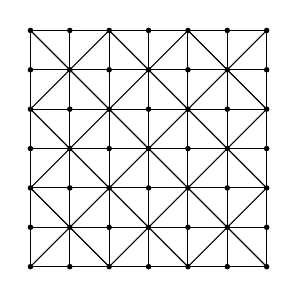
\begin{tikzpicture}[scale=0.5]
        % Define the size of the grid
\def\n{7}

\foreach \j in {0,...,\numexpr\n-1} {
    \foreach \i in {0,...,\numexpr\n-1} {
        \fill (\i,\j) circle[radius=2pt];  % black filled circle
    }
}

\foreach \j in {0,...,\numexpr\n-2} {
    \foreach \i in {0,...,\numexpr\n-1} {
        \draw (\i,\j) -- (\i,\j+1);
    }
}

\foreach \j in {0,...,\numexpr\n-1} {
    \foreach \i in {0,...,\numexpr\n-2} {
        \draw (\i,\j) -- (\i+1,\j);
    }
}

\foreach \j in {0,...,\numexpr\n-2} {
    \foreach \i in {0,...,\numexpr\n-2} {
        \pgfmathtruncatemacro{\sumval}{\i + \j}
        \ifthenelse{\isodd{\sumval}}
        {
            \draw (\i+1,\j) -- (\i,\j+1);
        }
        {
            \draw (\i,\j) -- (\i+1,\j+1);
        }
    }
}

    \end{tikzpicture}
    \caption{Pattern 1 of graphs for a grid of \(7 \times 7\) vertices}
    \label{fig:graph_pattern_1}
\end{figure}


\begin{figure}
    \centering
    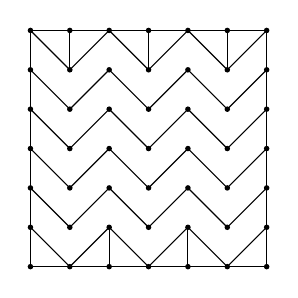
\begin{tikzpicture}[scale=0.5]
        % Define the size of the grid
\def\n{7}

\foreach \j in {0,...,\numexpr\n-1} {
    \foreach \i in {0,...,\numexpr\n-1} {
        \fill (\i,\j) circle[radius=2pt];  % black filled circle
    }
}

% Vertical lines on left and right edges
\foreach \j in {0,...,\numexpr\n-2} {
    \draw (0,\j) -- (0,\j+1);
    \draw (\numexpr\n-1,\j) -- (\numexpr\n-1,\j+1);
    
    \foreach \i in {0,...,\numexpr\n-2} {
        \ifthenelse{\isodd{\i}}{
            \draw (\i,\j) -- (\i+1,\j+1);
        }{
            \ifthenelse{\j > 0}{
                \draw (\i,\j) -- (\i+1,\j-1);
            }{}
        }
    }
}

% Horizontal lines on top and bottom edges
\foreach \i in {0,...,\numexpr\n-2} {
    \draw (\i,0) -- (\i+1,0);
    \draw (\i,\numexpr\n-1) -- (\i+1,\numexpr\n-1);
    
    \ifthenelse{\isodd{\i}=0}{
        \draw (\i-1,\numexpr\n-1) -- (\i,\numexpr\n-2);
    }{}
    
    \ifthenelse{\i > 0}{
        \ifthenelse{\isodd{\i}=0}{
            \draw (\i,\numexpr\n-2) -- (\i,\numexpr\n-1);
        }{
            \draw (\i,0) -- (\i,1);
        }
    }{}
}
    \end{tikzpicture}
    \caption{Pattern 2 of graphs for a grid of \(7 \times 7\) vertices}
    \label{fig:graph_pattern_2}
\end{figure}

\begin{figure}
    \centering
    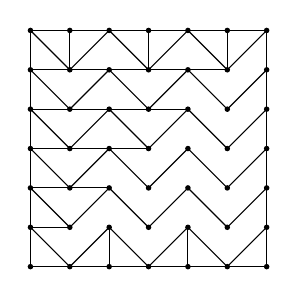
\begin{tikzpicture}[scale=0.5]
        % Define the size of the grid
\def\n{7}

\foreach \j in {0,...,\numexpr\n-1} {
    \foreach \i in {0,...,\numexpr\n-1} {
        \fill (\i,\j) circle[radius=2pt];  % black filled circle
    }
}

% Vertical lines on left and right edges
\foreach \j in {0,...,\numexpr\n-2} {
    \draw (0,\j) -- (0,\j+1);
    \draw (\numexpr\n-1,\j) -- (\numexpr\n-1,\j+1);
    
    \foreach \i in {0,...,\numexpr\n-2} {
        \ifthenelse{\isodd{\i}}{
            \draw (\i,\j) -- (\i+1,\j+1);
        }{
            \ifthenelse{\j > 0}{
                \draw (\i,\j) -- (\i+1,\j-1);
            }{}
        }
    }
}

% Horizontal lines on top and bottom edges
\foreach \i in {0,...,\numexpr\n-2} {
    \draw (\i,0) -- (\i+1,0);
    \draw (\i,\numexpr\n-1) -- (\i+1,\numexpr\n-1);
    
    \ifthenelse{\isodd{\i}=0}{
        \draw (\i-1,\numexpr\n-1) -- (\i,\numexpr\n-2);
    }{}
    
    \ifthenelse{\i > 0}{
        \ifthenelse{\isodd{\i}=0}{
            \draw (\i,\numexpr\n-2) -- (\i,\numexpr\n-1);
        }{
            \draw (\i,0) -- (\i,1);
        }
    }{}
}

% Outer loop: j from 1 to n-2
\foreach \j in {1,...,\numexpr\n-2} {
    % Inner loop: i from 0 to j-1 (since range(0, j))
    \foreach \i in {0,...,\numexpr\j-1} {
        % Draw line from (i, j) to (i+1, j)
        \draw (\i,\j) -- (\numexpr\i + 1,\j);
    }
}

% Draw grid lines
  % \draw[gray, dotted] (0, 0) grid (\numexpr\n-1, \numexpr\n-1);

    \end{tikzpicture}
    \caption{Pattern 3 of graphs for a grid of \(7 \times 7\) vertices}
    \label{fig:graph_pattern_3}
\end{figure}



\captionsetup[table]{skip=10pt}

\begin{table*}
\centering
\begin{tabularx}{\textwidth}{|X|X|X|X|X|X|}
% \begin{tabularx}{\textwidth}{|C|C|C|C|C|C|}
\hline
Graph ID & Pattern Grid Side Length \((l)\) & Pattern Type & Number of Vertices \((n)\) & Number of Edges \((m)\) & Number of Regions \\
\hline
\(g_1\) & 1,001 & \(P_1\) & 1,002,001 & 3,002,000 & 2,000,001 \\
\hline
\(g_2\) & 1,001 & \(P_2\) & 1,002,001 & 1,004,999 & 3,000 \\
\hline
\(g_3\) & 1,001 & \(P_3\) & 1,002,001 & 1,504,499 & 502,500 \\
\hline
\(g_4\) & 4,001 & \(P_1\) & 16,008,001 & 48,008,000 & 32,000,001 \\
\hline
\(g_5\) & 4,001 & \(P_2\) & 16,008,001 & 16,019,999 & 12,000 \\
\hline
\(g_6\) & 4,001 & \(P_3\) & 16,008,001 & 24,017,999 & 8,010,000 \\
\hline
\(g_7\) & 8,001 & \(P_1\) & 64,016,001 & 192,016,000 & 128,000,001 \\
\hline
\(g_8\) & 8,001 & \(P_2\) & 64,016,001 & 64,039,999 & 24,000 \\
\hline
\(g_9\) & 8,001 & \(P_3\) & 64,016,001 & 96,035,999 & 32,020,000 \\
\hline
\(g_{10}\) & 12,001 & \(P_1\) & 144,024,001 & 432,024,000 & 288,000,001 \\
\hline
\(g_{11}\) & 12,001 & \(P_2\) & 144,024,001 & 144,059,999 & 36,000 \\
\hline
\(g_{12}\) & 12,001 & \(P_3\) & 144,024,001 & 216,053,999 & 72,030,000 \\
\hline

\end{tabularx}
\caption{Graphs Data for Different Patterns and Sizes}
\label{tab:graph_data}
\end{table*}

\subsection{Results}

% For the different graphs mentioned in the table~\ref{tab:graph_data}, regions are extracted using the different CPU methods mentioned above (BGL, CGAL, and the original algorithm implemented on the CPU), and the time and the results are compared to the GPU implementation. The correctness is tested across the graphs, and the time speedup was calculated as the ratio between the GPU implementation time and the other CPU implementations time. As mentioned before, the time is calculated for the group of the graph with the smallest \(l\) where \(l = 1001\) for the BGL implementation. You can find the results in table~\ref{tab:results}. You can see from the table that the fastest CPU implementation is for our own C++ code, because it executes only the algorithm and doesn't do any planarity checks, and this is useful in our case, and as a result, we will focus on the comparison between it and the CUDA implementation. Figure~\ref{fig:speedup} illustrates the speedup between our CPU and the GPU implementations of the algorithm, where you can see that the speedup is increasing for larger graphs till it reaches $33\times$ for the largest graphs with an average speedup 50x. The resulting speedup values show the importance of using the GPU implementation.

For the graph instances listed in Table~\ref{tab:graph_data}, region extraction was performed using the four CPU-based approaches described above: BGL, CGAL libraries, and our own C++ implementations of the Wedge-based and the HE-based algorithms, and 2 GPU-based approaches, the Wedge-based and the HE-based. Correctness was verified across all graph instances, and the speedup of each implementation was computed as the ratio of the execution time to the HE-based GPU execution time, as the fastest run time results were for the HE-based algorithm either on the CPU or on the GPU for most of the test cases. It is noted that the GPU-accelerated HE-based algorithm is slightly faster than the GPU-accelerated Wedge-based algorithm. 

As mentioned previously, for the BGL implementation, timing measurements were limited to the smallest graph group ($l = 1001$), due to the overhead associated with planarity testing. The detailed results are presented in Table~\ref{tab:results}. Among the CPU approaches, our HE-based C++ implementation achieved better performance than the libraries, as it executes only the core algorithm without performing planarity checks, and better than the Wedge-based implementation, which was expected because it depends on the twin edges to find the next edges, and it does not need to do binary search. Comparing the two parallel approaches shows that the Half-Edge implementation consistently outperforms the Wedge-based framework. This advantage arises because the Half-Edge data structure tracks connectivity natively, avoiding the secondary wedge-sorting step required by the wedge algorithm, with the latter typically being up to 13\% slower across test cases. Consequently, the primary comparison focuses on this CPU implementation and the CUDA-based GPU implementation for the HE-based algorithm which are the fastest CPU and GPU implementations.

Figure~\ref{fig:speedup} illustrates the resulting speedup, demonstrating a clear increase in performance gains as the graph size grows. The speedup reaches up to $33\times$ for the largest graph instances, with an average speedup of $23.7\times$. These results highlight the significant performance benefits of the GPU-based implementation. Pattern 1 exhibits lower speedup due to significant load imbalance caused by its non-uniform region distribution. The algorithm's parallel efficiency depends on the maximum region size; since Pattern 1 is dominated by one massive exterior region (with size $4(l+1)$) alongside many small triangular regions, GPU threads must wait for the largest region to process. High speedup is more readily achieved in patterns where region sizes are homogeneous, ensuring a balanced workload.

% The reason why the speedup of pattern 1 is much less than the other patterns is that pattern 1 has only 1 large region (the exterior region with size $4(l+1)$ and all the other regions are triangular, and the parallel algorithm performance depends on the largest region size. The more the regions size is close to each other, the more speedup is achieved.

\captionsetup[table]{skip=10pt}

% \begin{table*}[t]
% \centering
% \begin{tabularx}{\textwidth}{|X|X|X|X|X|X|X|X|X|X|X|X|}
% \hline
% \textbf{Graph ID} & \textbf{GPU-HE Time (s)} & \textbf{GPU-Wedge Time (s)} & \textbf{Speedup} & \textbf{CPU-HE Time (s)} & \textbf{Speedup} & \textbf{CPU-Wedge Time (s)} & \textbf{Speedup} & \textbf{CGAL Time (s)} & \textbf{Speedup} & \textbf{BGL Time (s)} & \textbf{Speedup} \\
% \hline
% \(g_1\) & 0.0126 & 0.0126 & 1 & 0.315 & 24.887 & 1.032 & 81.49 & 5.01 & 395.7 & 1.55 & 122.517 \\
% \hline
% \(g_2\) & 0.00675 & 0.00715 & 1.06 & 0.155 & 22.977 & 0.469 & 69.429 & 2.395 & 354.798 & 1.112 & 164.725 \\
% \hline
% \(g_3\) & 0.0088 & 0.0098 & 1.0584 & 0.223 & 25.21 & 0.651 & 73.67 & 3.027 & 342.54 & 1.69 & 191 \\
% \hline
% \(g_4\) & 0.398 & 0.4316 & 1.086 & 5.207 & 13.098 & 18.093 & 45.509 & 92.46 & 232.57 & N/A & N/A \\
% \hline
% \(g_5\) & 0.13 & 0.142 & 1.093 & 3.31 & 25.472 & 8.83 & 67.911 & 42.93 & 330.302 & N/A & N/A \\
% \hline
% \(g_6\) & 0.179 & 0.195 & 1.094 & 4.69 & 26.269 & 12.74 & 71.344 & 56.43 & 316.037 & N/A & N/A \\
% \hline
% \(g_7\) & 1.577 & 1.72 & 1.092 & 21.13 & 13.39 & 75.26 & 47.71 & 417.035 & 264.37 & N/A & N/A \\
% \hline
% \(g_8\) & 0.496 & 0.551 & 1.11 & 15.578 & 31.4 & 39.9 & 80.47 & 179.22 & 361.26 & N/A & N/A \\
% \hline
% \(g_9\) & 0.77 & 0.84 & 1.09 & 20.85 & 27.2 & 56 & 72.73 & 243.38 & 317.45 & N/A & N/A \\
% \hline
% \(g_{10}\) & 3.52 & 3.85 & 1.1 & 47.99 & 13.64 & 173.29 & 49.23 & 1026.41 & 291.59 & N/A & N/A \\
% \hline
% \(g_{11}\) & 1.09 & 1.23 & 1.13 & 36.15 & 33.216 & 97.82 & 89.88 & 441.28 & 404.84 & N/A & N/A \\
% \hline
% \(g_{12}\) & 1.7 & 1.89 & 1.11 & 47.9 & 28.13 & 131.42 & 77.16 & 612 & 360 & N/A & N/A \\
% \hline

% \end{tabularx}
% \caption{Experimental results for regions extraction of the different graphs using the different implementations and the speedup against the HE-based GPU implementation time}
% \label{tab:results}
% \end{table*}


\begin{table*}
\centering
\small % Slightly smaller font to help 12 columns fit better
\begin{tabularx}{\textwidth}{|X|>{\columncolor[gray]{0.9}}X|X|X|>{\columncolor[gray]{0.9}}X|X|X|X|X|X|X|X|}
\hline
Graph ID & GPU-HE Time (s) & GPU-Wedge Time (s) & Speedup of GPU-HE & CPU-HE Time (s) & Speedup of GPU-HE & CPU-Wedge Time (s) & Speedup of GPU-HE & CGAL Time (s) & Speedup of GPU-HE & BGL Time (s) & Speedup of GPU-HE \\
\hline
\(g_1\) & 0.0126 & 0.0126 & 1.00 & 0.315 & 25.00 & 1.032 & 81.90 & 5.01 & 397.62 & 1.55 & 123.02 \\
\hline
\(g_2\) & 0.00675 & 0.00715 & 1.06 & 0.155 & 22.96 & 0.469 & 69.48 & 2.395 & 354.81 & 1.112 & 164.74 \\
\hline
\(g_3\) & 0.0088 & 0.0098 & 1.11 & 0.223 & 25.34 & 0.651 & 73.98 & 3.027 & 343.98 & 1.69 & 192.05 \\
\hline
\(g_4\) & 0.398 & 0.4316 & 1.08 & 5.207 & 13.08 & 18.093 & 45.46 & 92.46 & 232.31 & N/A & N/A \\
\hline
\(g_5\) & 0.13 & 0.142 & 1.09 & 3.31 & 25.46 & 8.83 & 67.92 & 42.93 & 330.23 & N/A & N/A \\
\hline
\(g_6\) & 0.179 & 0.195 & 1.09 & 4.69 & 26.20 & 12.74 & 71.17 & 56.43 & 315.25 & N/A & N/A \\
\hline
\(g_7\) & 1.577 & 1.72 & 1.09 & 21.13 & 13.40 & 75.26 & 47.72 & 417.035 & 264.45 & N/A & N/A \\
\hline
\(g_8\) & 0.496 & 0.551 & 1.11 & 15.578 & 31.41 & 39.9 & 80.44 & 179.22 & 361.33 & N/A & N/A \\
\hline
\(g_9\) & 0.77 & 0.84 & 1.09 & 20.85 & 27.08 & 56.0 & 72.73 & 243.38 & 316.08 & N/A & N/A \\
\hline
\(g_{10}\) & 3.52 & 3.85 & 1.09 & 47.99 & 13.63 & 173.29 & 49.23 & 1026.41 & 291.59 & N/A & N/A \\
\hline
\(g_{11}\) & 1.09 & 1.23 & 1.13 & 36.15 & 33.17 & 97.82 & 89.74 & 441.28 & 404.84 & N/A & N/A \\
\hline
\(g_{12}\) & 1.7 & 1.89 & 1.11 & 47.9 & 28.18 & 131.42 & 77.31 & 612.0 & 360.00 & N/A & N/A \\
\hline
\end{tabularx}
\caption{Experimental results for regions extraction of the different graphs using the different implementations and the speedup of the HE-based GPU implementation time against the different implementations.}
\label{tab:results}
\end{table*}

\begin{figure}
\centering
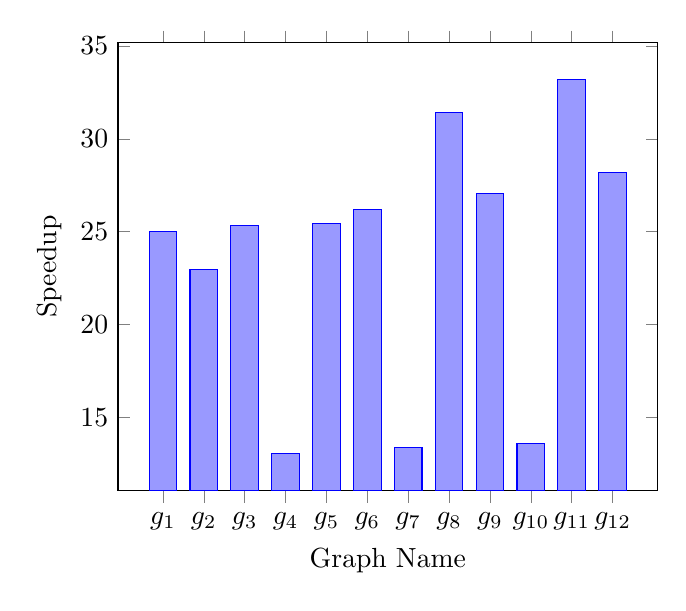
\begin{tikzpicture}
\begin{axis}[
    ybar,                   % Single series vertical bars chart
    ylabel={Speedup},
    xlabel={Graph Name},
    xtick=data,
    symbolic x coords={
        \(g_1\), \(g_2\), \(g_3\), \(g_4\), \(g_5\), \(g_6\), \(g_7\), \(g_8\), \(g_9\), \(g_{10}\), \(g_{11}\), \(g_{12}\) 
    },
]

\addplot[fill=blue!40, draw=blue] coordinates {
    (\(g_1\), 25.00) (\(g_2\), 22.96) (\(g_3\), 25.34) 
    (\(g_4\), 13.08) (\(g_5\), 25.46) (\(g_6\), 26.20)
    (\(g_7\), 13.40) (\(g_8\), 31.41) (\(g_9\), 27.08)
    (\(g_{10}\), 13.63) (\(g_{11}\), 33.17) (\(g_{12}\), 28.18)
};

\end{axis}
\end{tikzpicture}
\caption{Speedup between the fastest CPU and the GPU implementations on different graphs (the HE-based implementations)}
\label{fig:speedup}
\end{figure}

\section{Conclusion}
In this work, we proposed two efficient GPU-accelerated algorithms for region extraction in plane graphs. The practical implementations, developed in CUDA C++, are optimized through techniques such as pointer jumping and by leveraging established CUDA libraries, including the Thrust library. The 2 original sequential algorithms have the same run-time complexity $O(m \log m)$, but the HE-based one achieves better performance than the Wedge-based and between the two proposed GPU-accelerated algorithms, the algorithm that is based on the half-edges achieves better run-time than the Wedge-based algorithm. The fastest proposed approach achieves up to $33\times$ speedup compared to the fastest CPU-based implementations, enabling the extraction of planar graph regions for large-scale instances.

The GPU-accelerated method has broad applicability across multiple domains, including computer graphics, geographic information systems (GIS), VLSI circuit design, and robotics. Its advantages are particularly pronounced when processing extremely large graphs containing substantial numbers of vertices and edges.


%% Loading bibliography style file
%\bibliographystyle{model1-num-names}
\bibliographystyle{cas-model2-names}

% Loading bibliography database
\bibliography{references}


%\vskip3pt

% \bio{}
% Author biography without author photo.
% Author biography. Author biography. Author biography.
% Author biography. Author biography. Author biography.
% Author biography. Author biography. Author biography.
% Author biography. Author biography. Author biography.
% Author biography. Author biography. Author biography.
% Author biography. Author biography. Author biography.
% Author biography. Author biography. Author biography.
% Author biography. Author biography. Author biography.
% Author biography. Author biography. Author biography.
% \endbio

% \bio{figs/cas-pic1}
% Author biography with author photo.
% Author biography. Author biography. Author biography.
% Author biography. Author biography. Author biography.
% Author biography. Author biography. Author biography.
% Author biography. Author biography. Author biography.
% Author biography. Author biography. Author biography.
% Author biography. Author biography. Author biography.
% Author biography. Author biography. Author biography.
% Author biography. Author biography. Author biography.
% Author biography. Author biography. Author biography.
% \endbio

% \bio{figs/cas-pic1}
% Author biography with author photo.
% Author biography. Author biography. Author biography.
% Author biography. Author biography. Author biography.
% Author biography. Author biography. Author biography.
% Author biography. Author biography. Author biography.
% \endbio

\end{document}

